% tesesusp.cls, v-0.0.1

% Based on 'bntex2ppgsi.cls', 'abntex2.csl' and on USP guidelines to create
% thesis and dissertation documents.
% See <https://www.overleaf.com/project/64f7bdf1641ad4a3a8482800>
% and <https://teses.usp.br/index.php?option=com_content&
%      view=article&id=52&Itemid=67&lang=en>
% to learn more.

\clearpage

% ----------------------------------------------------------------------
% Cover (mandatory)
% ----------------------------------------------------------------------

\imprimircapa

% ----------------------------------------------------------------------
% Title page (mandatory)
% ----------------------------------------------------------------------

\imprimirfolhaderosto*

% ----------------------------------------------------------------------
% Cataloging record (mandatory)
% ----------------------------------------------------------------------

%% Do not use for qualification exams.
\begin{fichacatalografica}
 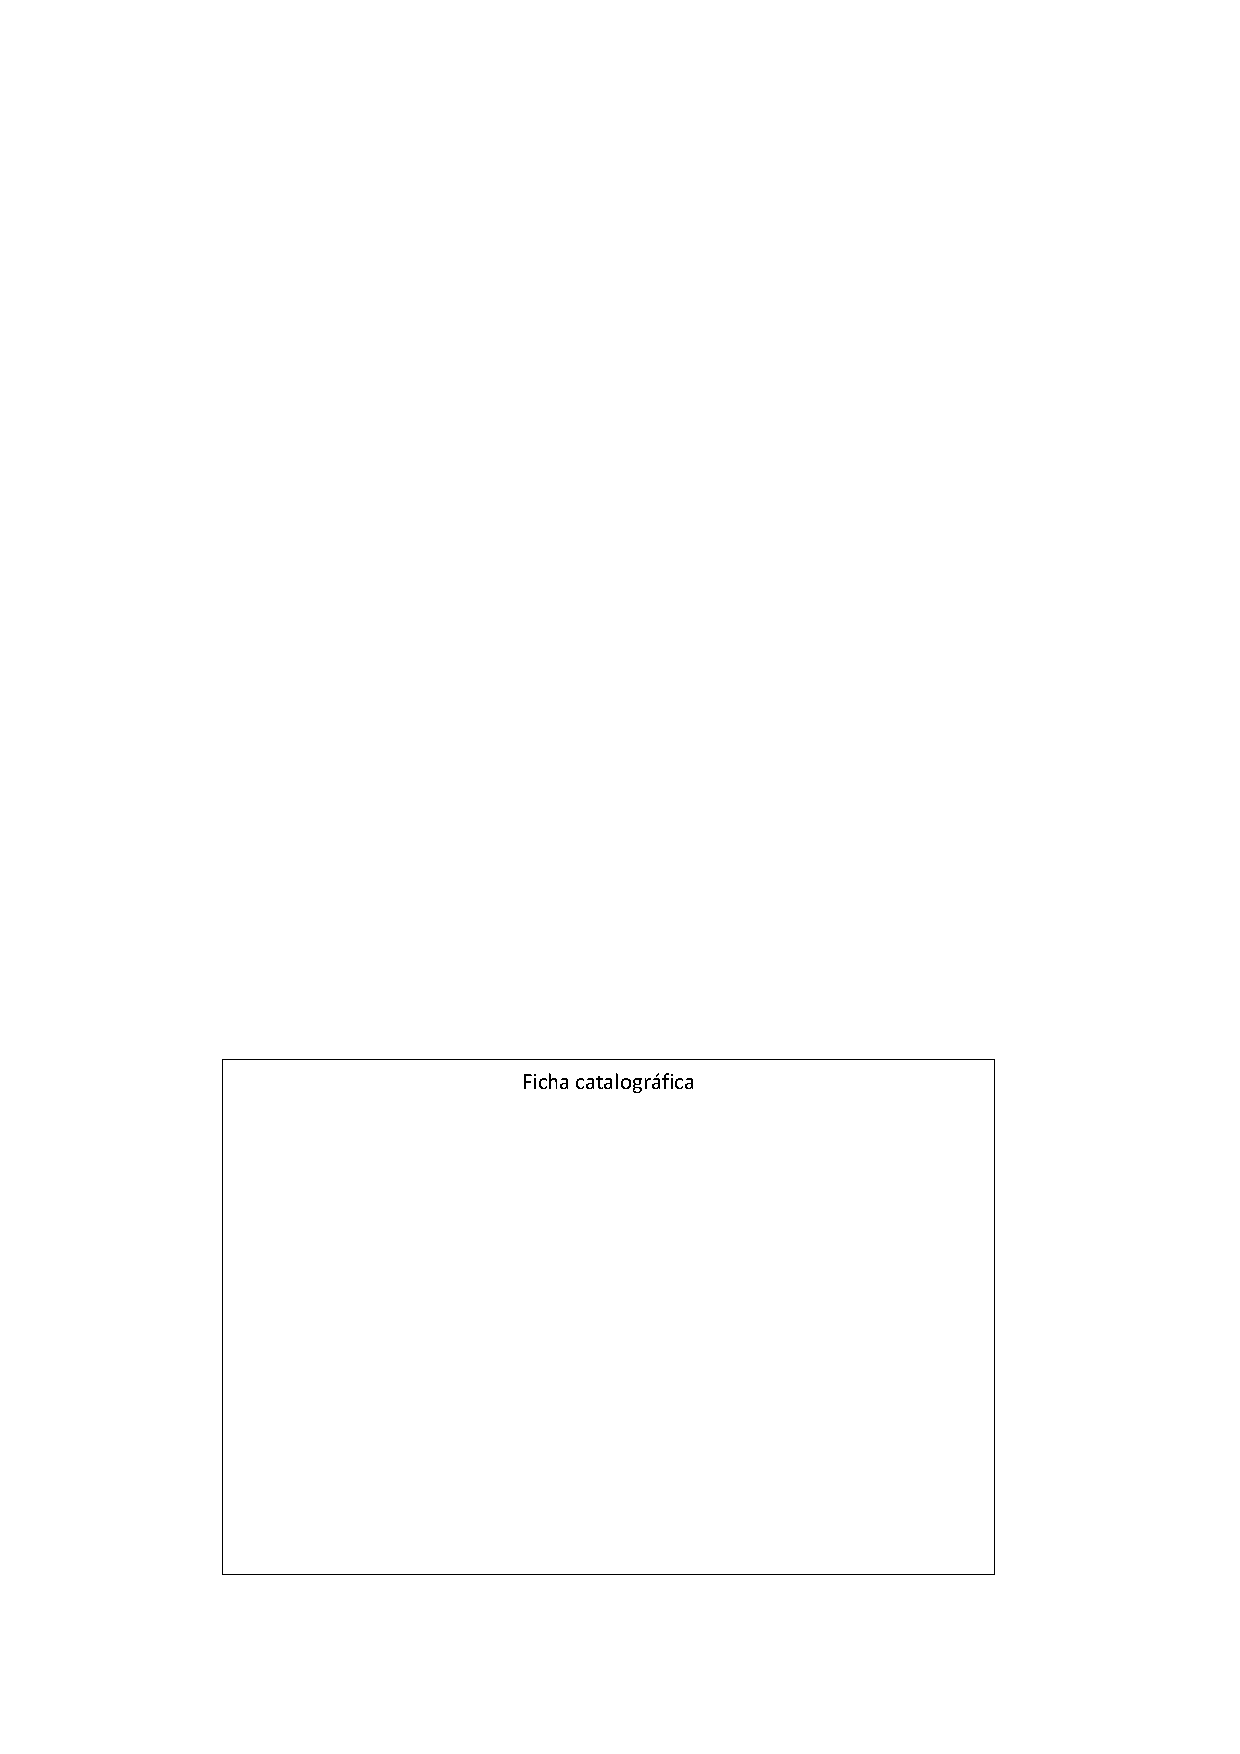
\includepdf{images/fig_ficha_catalografica.pdf}
\end{fichacatalografica}

% ----------------------------------------------------------------------
% Errata (optional)
% ----------------------------------------------------------------------

\begin{errata}
  This is the thesis development version (<1.0.0). Corrections will be listed here, if needed, after the thesis defense.
\end{errata}

% ----------------------------------------------------------------------
% Approval sheet (mandatory)
% ----------------------------------------------------------------------

\begin{folhadeaprovacao}

\noindent Qualifying exam text by [AUTHOR's FULL NAME], under the title \textbf{``\imprimirtitulo''}, presented to the School of Arts, Sciences, and Humanities at the University of São Paulo, as part of the requirements for the degree of [Master/PhD of Science] by the [GRADUATE PROGRAM], in the concentration area of [AREA], approved on \_\_\_\_\_\_\_\_\_\_\_\_\_\_ \_\_\_, \_\_\_\_\_\_, by the examining committee composed of the following doctors:

% \noindent Dissertation/Thesis by [AUTHOR's FULL NAME], sob o título \textbf{``\imprimirtitulo''}, presented to the School of Arts, Sciences, and Humanities at the University of São Paulo, as part of the requirements for the degree of [Master/PhD of Science] by the [GRADUATE PROGRAM], in the concentration area of [AREA], approved on \_\_\_\_\_\_\_\_\_\_\_\_\_\_ \_\_\_, \_\_\_\_\_\_, by the examining committee composed of the following doctors:

\vspace*{3cm}

\begin{center}

\_\_\_\_\_\_\_\_\_\_\_\_\_\_\_\_\_\_\_\_\_\_\_\_\_\_\_\_\_\_\_\_\_\_\_\_\_\_\_\_\_\_\_\_\_\_\_\_\_\_\_\_\_\_\_\_
\vspace*{0.2cm}
\\ \textbf{Prof. Dr. \_\_\_\_\_\_\_\_\_\_\_\_\_\_\_\_\_\_\_\_\_\_\_\_\_\_\_\_\_\_\_\_\_\_\_\_\_\_\_\_\_\_\_\_\_\_\_\_\_\_\_\_\_\_\_\_\_\_\_\_\_\_}
\\ \vspace*{0.2cm}
Instituição: \_\_\_\_\_\_\_\_\_\_\_\_\_\_\_\_\_\_\_\_\_\_\_\_\_\_\_\_\_\_\_\_\_\_\_\_\_\_\_\_\_\_\_\_\_\_\_\_\_\_\_\_\_\_\_\_\_\_
\\ \vspace*{0.2cm}
Presidente

\vspace*{2cm}

\_\_\_\_\_\_\_\_\_\_\_\_\_\_\_\_\_\_\_\_\_\_\_\_\_\_\_\_\_\_\_\_\_\_\_\_\_\_\_\_\_\_\_\_\_\_\_\_\_\_\_\_\_\_\_\_
\vspace*{0.2cm}
\\ \textbf{Prof. Dr. \_\_\_\_\_\_\_\_\_\_\_\_\_\_\_\_\_\_\_\_\_\_\_\_\_\_\_\_\_\_\_\_\_\_\_\_\_\_\_\_\_\_\_\_\_\_\_\_\_\_\_\_\_\_\_\_\_\_\_\_\_\_}
\\ \vspace*{0.2cm}
Instituição: \_\_\_\_\_\_\_\_\_\_\_\_\_\_\_\_\_\_\_\_\_\_\_\_\_\_\_\_\_\_\_\_\_\_\_\_\_\_\_\_\_\_\_\_\_\_\_\_\_\_\_\_\_\_\_\_\_\_

\vspace*{2cm}

\_\_\_\_\_\_\_\_\_\_\_\_\_\_\_\_\_\_\_\_\_\_\_\_\_\_\_\_\_\_\_\_\_\_\_\_\_\_\_\_\_\_\_\_\_\_\_\_\_\_\_\_\_\_\_\_
\vspace*{0.2cm}
\\ \textbf{Prof. Dr. \_\_\_\_\_\_\_\_\_\_\_\_\_\_\_\_\_\_\_\_\_\_\_\_\_\_\_\_\_\_\_\_\_\_\_\_\_\_\_\_\_\_\_\_\_\_\_\_\_\_\_\_\_\_\_\_\_\_\_\_\_\_}
\\ \vspace*{0.2cm}
Instituição: \_\_\_\_\_\_\_\_\_\_\_\_\_\_\_\_\_\_\_\_\_\_\_\_\_\_\_\_\_\_\_\_\_\_\_\_\_\_\_\_\_\_\_\_\_\_\_\_\_\_\_\_\_\_\_\_\_\_

\vspace*{2cm}

\_\_\_\_\_\_\_\_\_\_\_\_\_\_\_\_\_\_\_\_\_\_\_\_\_\_\_\_\_\_\_\_\_\_\_\_\_\_\_\_\_\_\_\_\_\_\_\_\_\_\_\_\_\_\_\_
\vspace*{0.2cm}
\\ \textbf{Prof. Dr. \_\_\_\_\_\_\_\_\_\_\_\_\_\_\_\_\_\_\_\_\_\_\_\_\_\_\_\_\_\_\_\_\_\_\_\_\_\_\_\_\_\_\_\_\_\_\_\_\_\_\_\_\_\_\_\_\_\_\_\_\_\_}
\\ \vspace*{0.2cm}
Instituição: \_\_\_\_\_\_\_\_\_\_\_\_\_\_\_\_\_\_\_\_\_\_\_\_\_\_\_\_\_\_\_\_\_\_\_\_\_\_\_\_\_\_\_\_\_\_\_\_\_\_\_\_\_\_\_\_\_\_

\end{center}
\end{folhadeaprovacao}

% ----------------------------------------------------------------------
% Inscription (optional)
% ----------------------------------------------------------------------

\begin{dedicatoria}
  \vspace*{\fill}
  \centering
  \noindent
  \textit{
    Write your inscription here, if desired, or remove this page.
  }
	\vspace*{\fill}
\end{dedicatoria}

% ----------------------------------------------------------------------
% Acknowledgments (optional)
% ----------------------------------------------------------------------

\begin{agradecimentos}
  I would like to acknowledge Daniel Vartanian's awesome \href{https://github.com/danielvartan/tesesusp}{Quarto format template}! :)
\end{agradecimentos}

% ----------------------------------------------------------------------
% Epigraph (optional)
% ----------------------------------------------------------------------

\begin{epigrafe}
  \vspace*{\fill}
	\begin{flushright}
	  \textit{
	    %% @theroyalsociety
		  ``Nullius in verba''\\ (The Royal Society, n.d.)
		}
	\end{flushright}
\end{epigrafe}

% ----------------------------------------------------------------------
% Abstract in the vernacular language (mandatory)
% ----------------------------------------------------------------------

\setlength{\absparsep}{18pt}
\begin{resumo}

\begin{flushleft}
[Sobrenome], [Iniciais]. ([Ano]). \textit{[Título]} [(Tese/Dissertação) de (Mestrado/Doutorado)]. [Departament/Escola], [Universidade], [Cidade]. [URL]
\end{flushleft}

Lorem ipsum dolor sit amet, consectetur adipiscing elit. Pellentesque accumsan rutrum lacus, vitae iaculis nisi bibendum in. Nulla et pellentesque nisl. Proin mollis dui sit amet egestas fermentum. Maecenas eu odio odio. Aenean porta ipsum in mauris pharetra dapibus. Nunc dapibus libero nec dui lacinia, id ultricies lectus maximus. Mauris quis mauris in velit pulvinar rutrum. Cras congue ante in orci luctus placerat. Nullam sit amet nisi augue. Maecenas non ligula eros. Etiam nec dolor a mi bibendum auctor.

Palavras-chaves: Palavra-chave 1. Palavra-chave 2. Palavra-chave 3.
\end{resumo}

% ----------------------------------------------------------------------
% % Abstract in the foreign language (mandatory)
% ----------------------------------------------------------------------

\begin{resumo}[Abstract]
\begin{otherlanguage*}{english}

\begin{flushleft}
[Surname], [Initials]. ([Year]). \textit{[Title]} [(Master's/PhD) thesis]. [Department/School], [University], [City]. [URL]
\end{flushleft}

Lorem ipsum dolor sit amet, consectetur adipiscing elit. Pellentesque accumsan rutrum lacus, vitae iaculis nisi bibendum in. Nulla et pellentesque nisl. Proin mollis dui sit amet egestas fermentum. Maecenas eu odio odio. Aenean porta ipsum in mauris pharetra dapibus. Nunc dapibus libero nec dui lacinia, id ultricies lectus maximus. Mauris quis mauris in velit pulvinar rutrum. Cras congue ante in orci luctus placerat. Nullam sit amet nisi augue. Maecenas non ligula eros. Etiam nec dolor a mi bibendum auctor.

Keywords: Keyword 1. Keyword 2. Keyword 3.
\end{otherlanguage*}
\end{resumo}

% ----------------------------------------------------------------------
% List of figures (optional)
% ----------------------------------------------------------------------

\pdfbookmark[0]{\listfigurename}{lof}
\listoffigures*
\cleardoublepage

% % ----------------------------------------------------------------------
% % List of algorithms (optional)
% % ----------------------------------------------------------------------
%
% \pdfbookmark[0]{\listalgorithmname}{loa}
% \listofalgorithms
% \cleardoublepage

% ----------------------------------------------------------------------
% List of tables (optional)
% ----------------------------------------------------------------------

\pdfbookmark[0]{\listtablename}{lot}
\listoftables*
\cleardoublepage

% ----------------------------------------------------------------------
% List of abbreviations and acronyms (optional)
% ----------------------------------------------------------------------

\begin{siglas}
  \item[Abbreviation 1] Abbreviation expanded definition
  \item[Abbreviation 2] Abbreviation expanded definition
  \item[Abbreviation 3] Abbreviation expanded definition
  \item[Abbreviation 4] Abbreviation expanded definition
  \item[Abbreviation 5] Abbreviation expanded definition
  \item[Abbreviation 6] Abbreviation expanded definition
  \item[Abbreviation 7] Abbreviation expanded definition
  \item[Abbreviation 8] Abbreviation expanded definition
  \item[Abbreviation 9] Abbreviation expanded definition
  \item[Abbreviation 10] Abbreviation expanded definition
\end{siglas}

% ----------------------------------------------------------------------
% List of symbols (optional)
% ----------------------------------------------------------------------

\begin{simbolos}
  \item[$ \Gamma $] Gamma
  \item[$ \Lambda $] Lambda
  \item[$ \zeta $] zeta
  \item[$ \in $] Belongs
\end{simbolos}

% ----------------------------------------------------------------------
% Table of contents (mandatory)
% ----------------------------------------------------------------------

\pdfbookmark[0]{\contentsname}{toc}
% \tableofcontents*
\cleardoublepage
